\chapter{Background}
\label{chap:background}

%\todo{Should information about the Vekveselva be included, or is it simply no interesting / important?}

\section{Immersive Virtual Field Trip for Field Course in Physical Geography}
    \label{sec:specialisation}
    This master's thesis builds on a specialisation project \cite{specialisation} that was done the previous (autumn) semester. Many preparations to this project was performed in that project. It started of with a literature review and joining the actual field trip to get the experience and take 360$^\circ$ degree images. The project also researched into recreating topology from LiDAR scans. In the end a simple prototype was created and evaluated by domain experts in geography.

\section{Theory and Technology}
    % About technology, both software and hardware that is currently on the market
    A literature review of the theory and technology of the field was conducted in the Specialisation Project that this master's thesis continue from. The following section is therefore directly extracted from said project\cite{specialisation}, with the exception of \cref{sec:threei}, \cref{sec:league} and \cref{sec:summary}\todo{Fill in cref} that have been added.
    
    \subsection{Different Types of Realities}
        % Continuum between real and virtual environment
        % Subgenres of extended reality XR
        When discussing different types of environments, it is natural to bring up the \emph{Reality - Virtuality continuum} \cite{reality_virtuality_continuum} as seen in \cref{fig:reality_virtuality_continuum}. This continuum was proposed in a paper by \emph{Paul Milgram} et al, discussing the different types of realities and environments.
        
        \begin{figure}[!ht]
            \centering
            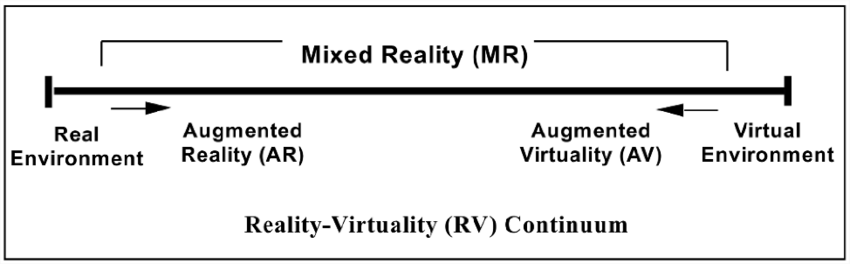
\includegraphics[width=\linewidth]{figures/reality_virtuality_continuum.png}
            \caption{The Reality - Virtuality Continuum}
            \label{fig:reality_virtuality_continuum}
        \end{figure}
        
        The continuum describes a continuous transition from the Real Environment, through the Mixed Reality into the Virtual Environment. Within the Mixed Reality there are two opposite realities: Augmented Reality (AR) and Augmented Virtuality (AV). Both include objects from the Real- and Virtual Environment, but differ in that AR is mainly the Real Environment with elements from the Virtual Environment, whereas AV is mainly the Virtual Environment with elements from the Real Environment. Because the transition is continuous it can become difficult to separate classify a reality as either AR or AV if it falls in between.
        
        \emph{Extended Reality} (XR) has been made as an umbrella term that incorporates both Mixed Reality and Virtual Reality \cite{xr}. This has been done to make a separation between the Real Environment and the rest that have some form of technology involved. The hierarchical relations of the different realities and environments have been illustrated in \cref{fig:xr}.
        
        \FloatBarrier
        \begin{figure}[!ht]
            \centering
            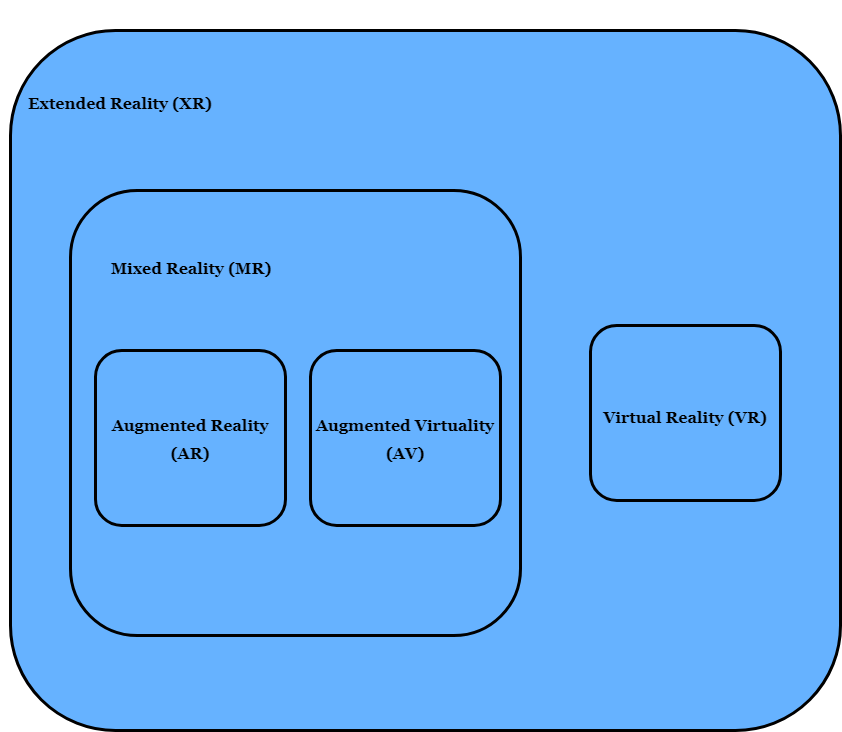
\includegraphics[width=0.7\linewidth]{figures/XR.png}
            \caption{Categories of Extended Reality}
            \label{fig:xr}
        \end{figure}
        \FloatBarrier
        
        As the Virtual Field Trip is planned to rely on a Head Mounted Display and the Omnidirectional Treadmill without using real elements directly, it will fall under the category of VR.
    
    \subsection{Virtual Reality}
        Even though Virtual Reality (VR) has become part of the mainstream media market, a brief introduction and evaluation is presented here.
        
        According to the Oxford Dictionary \cite{oxford}, VR is:
        
        \begin{quote}
            \textit{''The computer-generated simulation of a three-dimensional image or environment that can be interacted with in a seemingly real or physical way by a person using special electronic equipment, such as a helmet with a screen inside or gloves fitted with sensors.''}
        \end{quote}
        
        Another dictionary, Merriam Webster \cite{merrian_webster}, defines VR as:
        
        \begin{quote}
            \textit{''An artificial environment which is experienced through sensory stimuli (such as sights and sounds) provided by a computer and in which one's actions partially determine what happens in the environment''}
        \end{quote}
        
        In the book \emph{The VR Book} by Jason Jerald \cite{the_vr_book}, VR is defined as:
        
        \begin{quote}
            \textit{''[...] a computer-generated digital environment that can be experienced and interacted with as if that environment were real.''}
        \end{quote}
        
        The definitions start to paint a picture of VR. A common denominator between these is a \textbf{computer-generated environment}. Furthermore they all agree on this environment being \textbf{interactive}.
        
            \subsubsection{The Three I's of VR}
                \label{sec:threei}
            
                \FloatBarrier
                \begin{figure}[htbp]
                    \centering
                    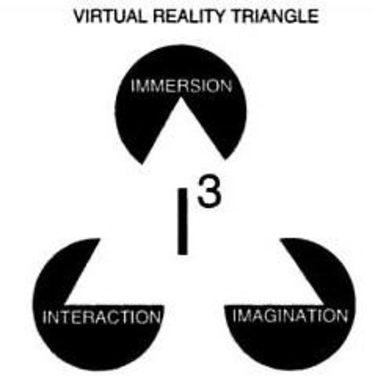
\includegraphics[width=0.5\linewidth]{figures/three_i.png}
                    \caption{The Three I's of Virtual Reality}
                    \label{fig:three_i}
                \end{figure}
                \FloatBarrier
                
                The term VR is also explored in the book \emph{Virtual Reality Technology}\cite{threei}. It is stated that VR has the three features: Immersion, Interaction and Imagination. As seen in \cref{fig:three_i}, the features are represented as equally important to the nature of VR. The book defines VR as:
                
                \begin{quote}
                    \textit{''Virtual reality is a high-end user-computer interface that involves real-time simulation and interactions through multiple sensorial channels. These sensorial modalities are visual, auditory, tactile, smell and taste.''}
                \end{quote}
                
                From this definition, the Immersion and Interaction feature of VR are clearly rooted. An important point made by the book is that VR should not be defined based on the devices that are used, but rather its purpose and function. The last feature, Imagination, is less obvious at first glance. Although not directly present in the quoted definition, VR is not only an interface, but has applications for real life problems. Because of this the imagination of the user is important for the performance of the simulation, and therefore the extent of which the application can solve a real problem. The imagination is also necessary to perceive non-existing things. This an important point as VR, although immersive, can not perfectly simulate the reality. The imagination bridges this gap by letting the user invest themselves in the simulated world, not unlike the suspension of disbelief when reading a book or watching a theatre play. This is demonstrated by the perceived, non-existing triangle in \cref{fig:three_i}.
                
            \subsubsection{VR Sickness}
                % Theories on why
                An unfortunate side effect that can arise from VR is VR sickness. VR sickness manifests itself in the same way as motion sickness, and can case nausea, vomiting and trouble maintaining balance \cite{motion_sickness}. According to researchers from the University of Newcastle Australia \cite{vr_sickness}, motion- and VR sickness might be the same thing, although other studies disagree. In the University of Newcastle study the researchers exposed volunteers to uncomfortable physical and visual tests and found large similarities in how the volunteers reacted. As the nature of VR- and motion sickness is still debated, there are a few theories to the cause of the problem \cite{vr_sickness_theories}:
                
                \begin{itemize}
                    \item \textbf{Sensory Conflict Theory} \\
                    This theory is the most widely accepted and states that the sickness is caused by a mismatch between visual and physical input. This happens when the eyes perceive motion, especially acceleration, and the body senses no force acting upon it.
                    
                    \SPACE
                
                    \item \textbf{Eye Movement Theory} \\
                    The theory suggests that the eyes move unnaturally compared to real life when viewing in \emph{Head Mounted Displays}. This happens because the images change differently to what the eyes expect and therefore strains the eyes, causing discomfort.
                    
                    \SPACE
                    
                    \item \textbf{Postural Instability Theory} \\
                    This theory builds on the theory that sickness occurs when animals are unable to keep their posture \cite{postural_instability}. On the assumption that this is correct, VR sickness is explained by small subconscious actions done to anticipate movement shown visually that is not present physically. These actions throw the user of balance, disrupting the posture and causing discomfort.
                    
                    \SPACE
                    
                    \item \textbf{Evolutionary Theory} \\
                    This is not as much a separate theory as more of a possible explanation of \emph{why} the sickness is present. It states that the symptoms are evolutionary reactions made to survive poisoning that can cause mismatch between visual and physical impressions, which is a common denominator in the different theories.
                \end{itemize}
                
                Regardless of the true reason for VR sickness, the theories provide similar ways to avoid it. The main points are to keep the players as stable as possible, avoiding acceleration and providing stable frames of references to help orient them.
            
        \subsection{VR, Learning and Engagement}
            As the presence of XR equipment increases, so too does the available research and experience with the technology. Several research papers have emerged that regard XR as improving learning outcome compared to traditional methods, like reading books and articles.
            
            A. Vishwanath et Al \cite{vr_low_income} studied the introduction of learning with VR by using Head Mounted Displays in a learning centre in a low income area in India. They worked with 16 students for several weeks, creating VR applications that covered several fields of study. They observed that the use of VR lead to the students displaying more curiosity in the field and being more inquisitive.
            
            D. M. Markowitz \cite{virtual_field_trips_learning} performed studies, field studies and experiments on over 270 students. They also noted that students were more curious after being exposed to VR learning applications as well as more knowledgeable. They also found a correlation between how much the students explored the space of the VR applications and how curious and inquisitive they became of the subject. This can be an indication that a more engaging experience offers better learning and sparks curiosity.
        
        \subsection{Head Mounted Displays}
            As the project will only include VR from the Reality - Virtuality Continuum, it will, as VR for the largest part does, be based on Head Mounted Displays. Generally speaking these are headsets that contain one or two screens and lenses capable of projecting individual images to each eye. The new application will use the HTC Vive Pro, whereas the Penn State application runs on the Oculus Go.
                
                \subsubsection{HTC Vive Pro}
                    This headset setup consists of two base stations, two controllers and the headset itself. The base stations are installed in a room to accurately track the players head and hand movements. It is not a stand-alone Head Mounted Display, and must therefore be connected and run on a computer. The headset has a resolution of 1440 x 1600 per eye on dual AMOLED screens, adding up to a total of 2880 x 1600. It Has a refresh rate of 90Hz and includes an integrated microphone and headphones. It won the award ''VR Headset of the year'' in 2018 and can be regarded as high-end hardware. \cite{vive_pro}
                    
                    \FloatBarrier
                    \begin{figure}[ht]
                        \centering
                        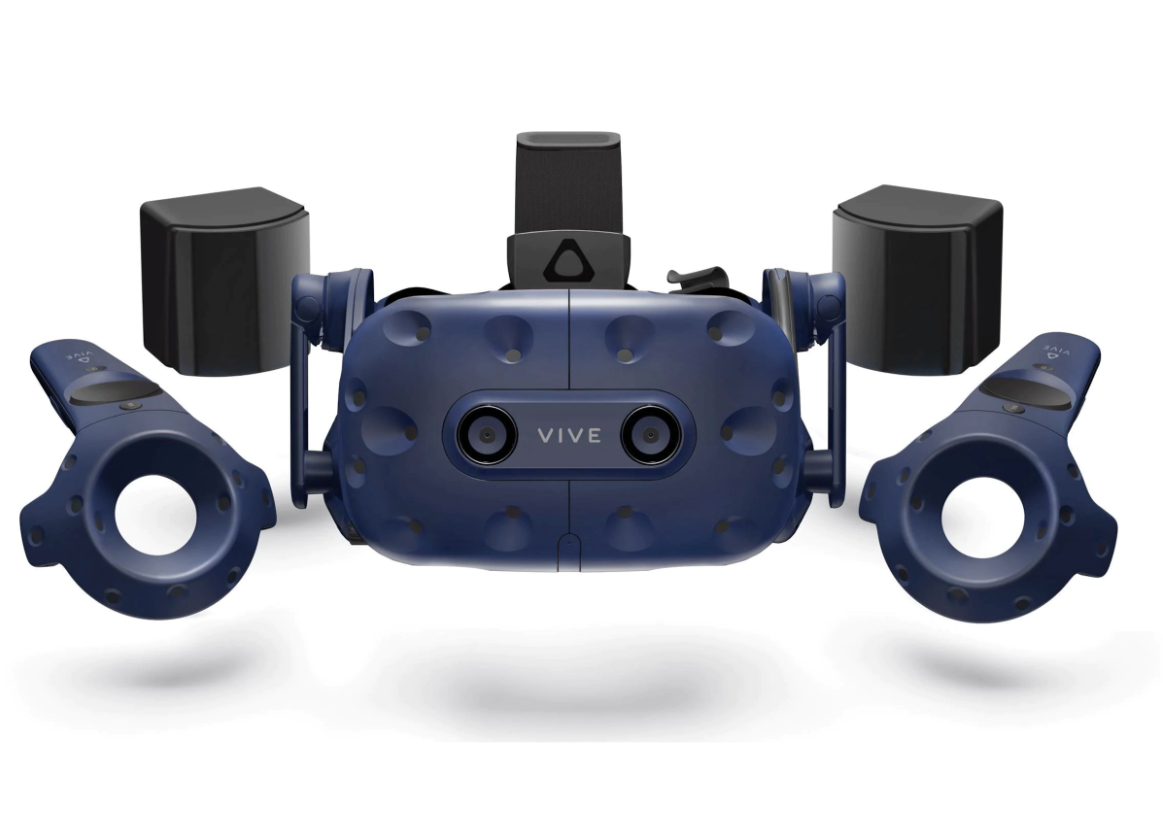
\includegraphics[width=0.9\linewidth]{figures/vive_pro.PNG}
                        \caption{The HTC Vive Pro Head Mounted Display with controllers and base stations}
                        \label{fig:vive_pro}
                    \end{figure}
                    \FloatBarrier
                    
                \subsubsection{Oculus Go}
                    In contrast to the HTC Vive Pro, the Oculus Go is a stand-alone Head Mounted Display, meaning that it has internal processors and does not need to be connected to a computer. It consist of one headset and one controller. It also has integrated speakers to offer an audible experience\cite{oculus_go}. This means that is a lot more portable and easier to set up, but at the cost of lower processing power and less accurate controller tracking. The Oculus has one 538 ppi\footnote{pixels per inch} screen with a resolution of 2560 x 1440\cite{oculus_specs}. It was launched in 2018, so it is from the same era as the HTC Vive Pro, but with a different purpose and price range.
                    
                    \FloatBarrier
                    \begin{figure}[ht]
                        \centering
                        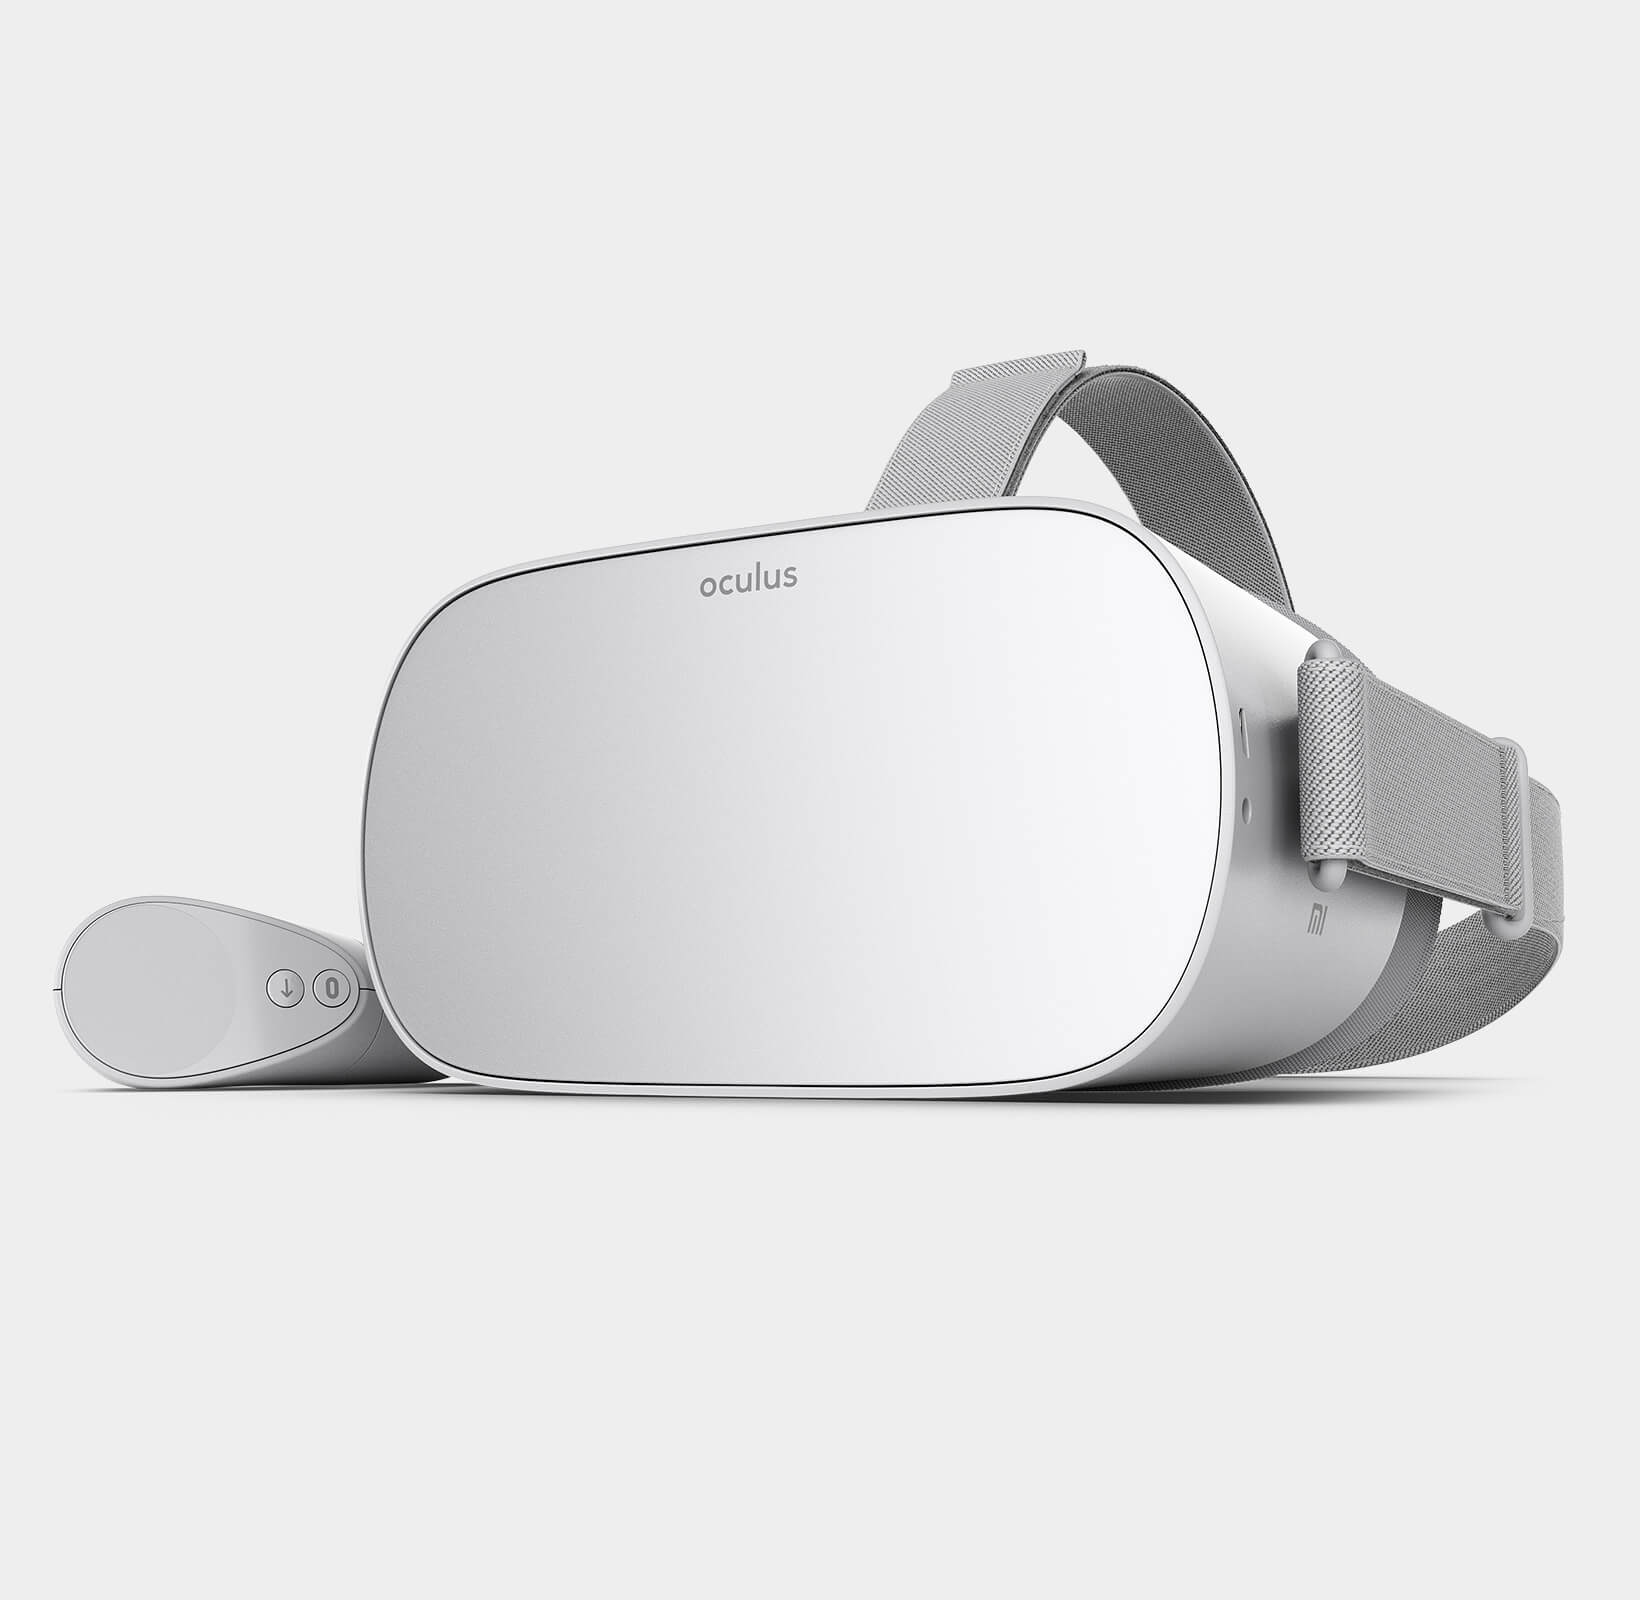
\includegraphics[width=0.9\linewidth]{figures/oculus_go.jpg}
                        \caption{The Oculus Go Head Mounted Display with its controller}
                        \label{fig:oculus_go}
                    \end{figure}
                    \FloatBarrier
            
            \subsection{Omnidirectional Treadmill}
            \label{sec:omni}
            
            \FloatBarrier
            \begin{figure}[htbp]
                \centering
                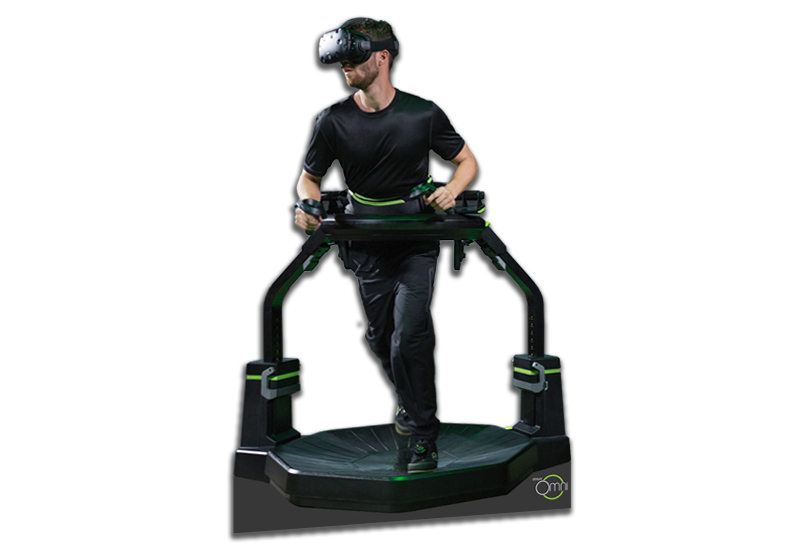
\includegraphics[width=0.9\linewidth]{figures/omni.png}
                \caption{Omni - the Omnidirectional Treadmill by Virtuix}
                \label{fig:omni}
            \end{figure}
            \FloatBarrier
            
            The Omni is an Omnidirectional Treadmill developed by Virtuix \cite{omni} and will be used as hardware for movement for the new application in the project. It is compatible with the HTC Vive Pro head mounted display. As illustrated in \cref{fig:omni} it consists of a concave surface, low friction shoe covers and a harness to keep the player in place. The Omni tracks the orientation of the player from the harness, as well as the feet movement by wireless sensors connected to the shoe covers. The movement of the feet is then transformed to in-game motion. The Omni can be used by an SDK\footnote{Software Development Kit} \cite{omni_sdk}, and Virtuix supplies SDKs for both the Unity and Unreal game engine. From Omni's web pages it can be seen that the applications featured are all of the entertaining type. This is indicative of it being mainly used for games and not for education.
    
    \subsection{Virtual Field Trips}
        \label{sec:vft}
        Virtual field trips are becoming more common in STEM\footnote{Science, Technology, Engineering and Math} education, where the areas of study that most implement the virtual field trips are geography, geoscience and architecture. Virtual Field Trips are, as the name implies, simulations of field trips meant to either support or replace the actual field trip. Even though they become more prominent, there are still numerous constraints to creating and using these applications. Many of the constraints revolve around the lack of tools that allow domain experts to create the virtual field trips themselves\cite{vft_geoscience}. Despite these challenges, some evidence point towards the virtual field trips having positive impacts on the courses. Research and experiments done by Kathy Jackson and more \cite{ivft_effectiveness} at Penn State University states that other research done on the effectiveness have shown inconsistent result, whereas they themselves found very positive impact on learning, enjoyment and grades. The inconsistent results can indicate that the topic needs more research.
        
        The researchers at Pennsylvania State University later compared three types of field trips: actual field trips (AFT), immersive virtual field trips (iVFT) using VR and desktop virtual field trips (dVFT)\cite{learning_in_the_field}. They found that the iVFT with VR was more engaging than it's desktop counterpart, but gave the same learning outcome. Curiously both the iVFT and dVFT scored better than the actual trip when measuring perceived learning outcomes. Their two key points out if these results are that VFTs can contribute positively to learning outcome, but does not necessarily have to be in VR.
        
        \todo{Talk about this in discussion}
        
        Similarly, research at Inland Norway University of Applied Sciences\cite{innland_university} investigated immersive virtual environments (IVEs). Immersive virtual environments are defined, by an article from two American universities investigating psychological experiments\cite{ive_definition}, so that \textit{"the user is perceptually surrounded by the VE (Virtual Environment"}. This is very similar to the definition of virtual reality, but with focus on the environment itself instead of the person's reality. It is also related to immersive virtual field trips that try to replicate real areas, but with learning as its main objective. The Inland researchers compared a real walk with a sitting VR application and a treadmill VR application. Their findings were that the sitting and treadmill VR applications performed similarly, but both suffered in enjoyment because of VR sickness. The immersive virtual environments still performed well on presence and replicating the real walk. This points to the quality of applications, and their ability to avoid vr sickness, to be and important challenge of immersive virtual environments and immersive virtual field trips.
        \cite{ive}
    
    \subsection{VR Virtual Field Trips}
        Virtual field trips are not necessarily in VR, but VR is the focus of this master's project. The current trend when it comes to the use of VR virtual field trips is to use low-level VR applications, meaning VR applications that run on low-cost hardware and that can be created with relatively low cost and effort\cite{vr_low_cost}. An opportunity that is present in these low cost VR applications is to have multiple users experiencing the field trip at once. This is something that can be taken into account when implementing non-low cost applications, as they will likely be used with an audience of other students.
    
    \subsection{Framework for Evaluating Virtual Field Trips}
        \label{sec:framework}
        In their research article, A. Klippel et al \cite{research_framework} propose a framework for assessing immersive learning experiences, specifically \emph{immersive Virtual Field Trips} (iVFTs). In essence this framework is a two-dimensional plane where one rates the VR technology on one axis and the content of the Virtual Field Trip on the other axis. An overview of the research framework is presented in \cref{fig:framework}
        
        \FloatBarrier
        \begin{figure}[!ht]
            \centering
            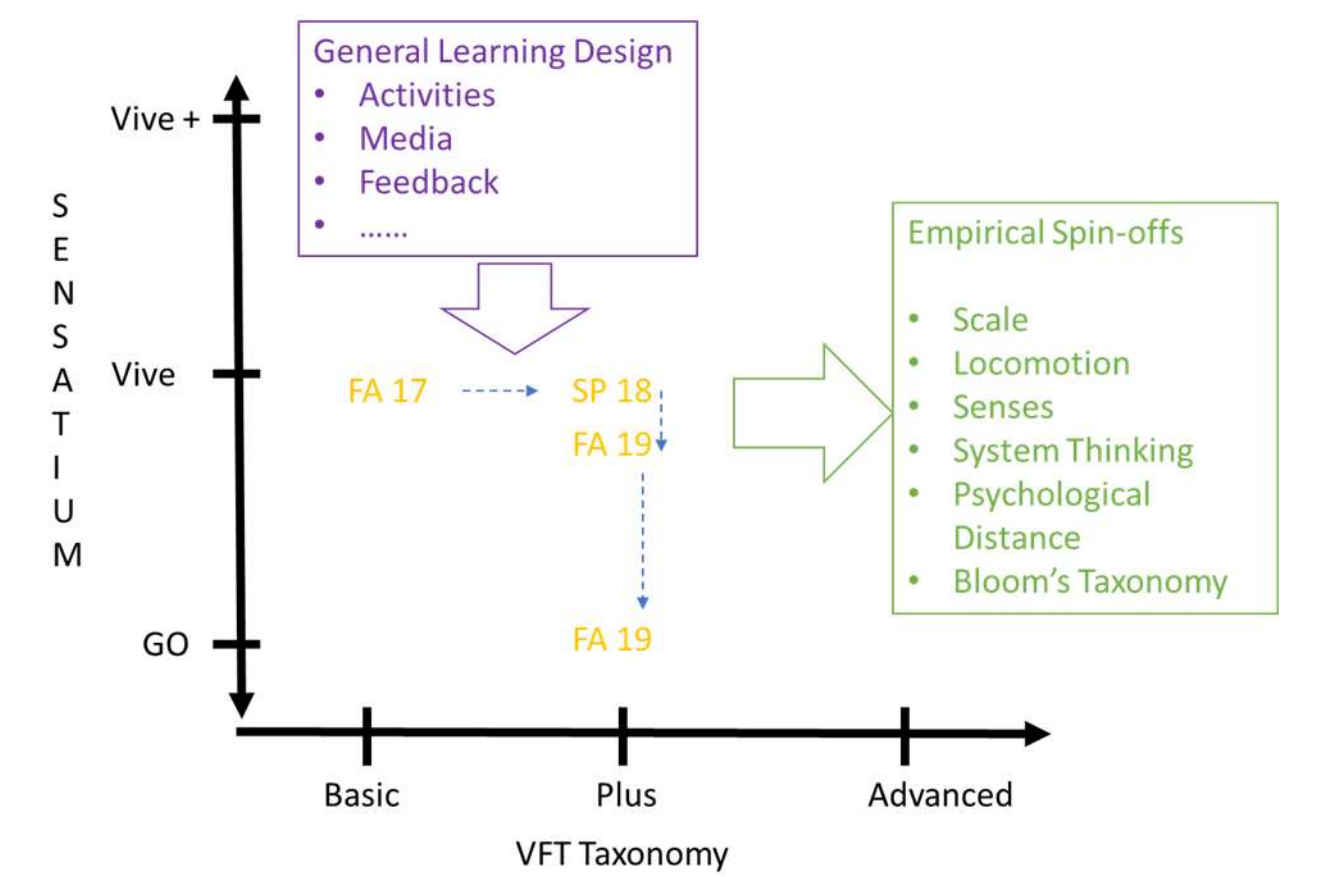
\includegraphics[width=0.7\linewidth]{figures/framework_3.PNG}
            \caption{Overview of the Research Framework for Immersive Virtual Field Trips}
            \label{fig:framework}
        \end{figure}
        \FloatBarrier
        
        On the left, vertical axis of the research framework overview (\cref{fig:framework}), the VR technology is evaluated. \emph{SENSATIUM} is a term coined by A. Klippel et al, which is an acronym for the \textbf{SEN}sing - \textbf{S}c\textbf{A}lability \textbf{T}rade - off cont\textbf{I}nu\textbf{UM}. As seen in \cref{fig:sensatium}, \emph{SENSATIUM} is a continuous scale where scalability goes from high to low, and sensing goes from low to high. Both are dependant on how advanced the equipment is. This shows that higher levels of sensing typically trades off against the ability to scale the application.
        
        \FloatBarrier
        \begin{figure}[!ht]
            \centering
            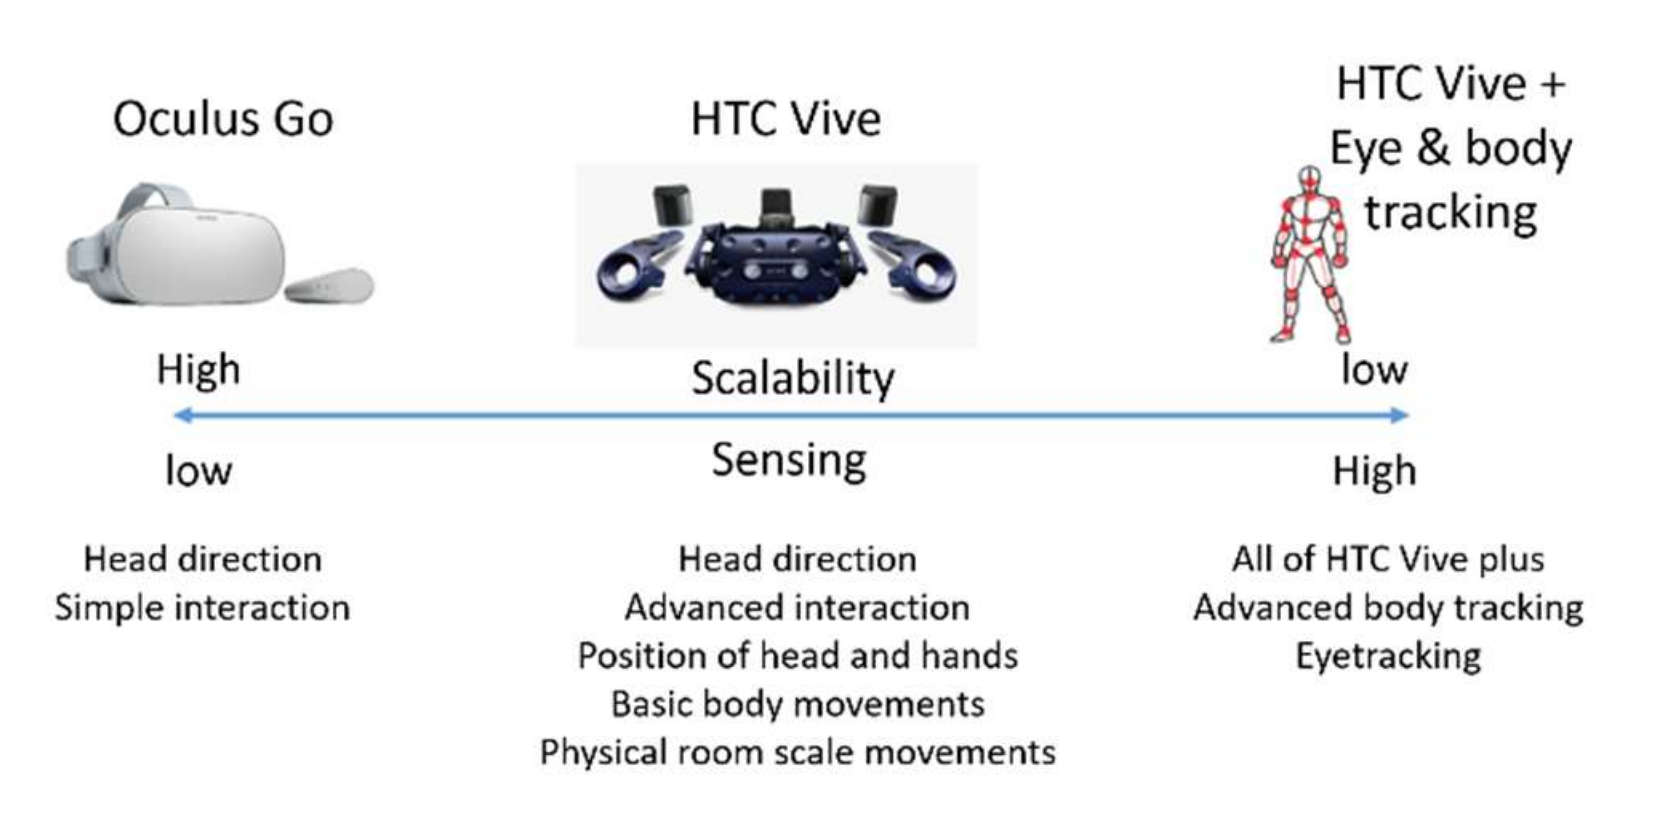
\includegraphics[width=0.7\linewidth]{figures/framework_technology_3.PNG}
            \caption{SENSATIUM, the \textbf{SEN}sing - \textbf{S}c\textbf{A}lability \textbf{T}rade - off cont\textbf{I}nu\textbf{UM}}
            \label{fig:sensatium}
        \end{figure}
        \FloatBarrier
        
        On the horizontal axis of the research framework overview (\cref{fig:framework}) the content of the immersive Virtual Field Trip is evaluated. The continuous scale goes from \emph{Basic}, through \emph{Plus} to \emph{Advanced}. This rating of immersive Virtual Field Trips, called the \emph{taxonomy} of immersive Virtual Field Trips, was also established by A. Klippel et al. The \emph{taxonomy} is explained in \cref{fig:taxonomy}
        
        \FloatBarrier
        \begin{figure}[!ht]
            \centering
            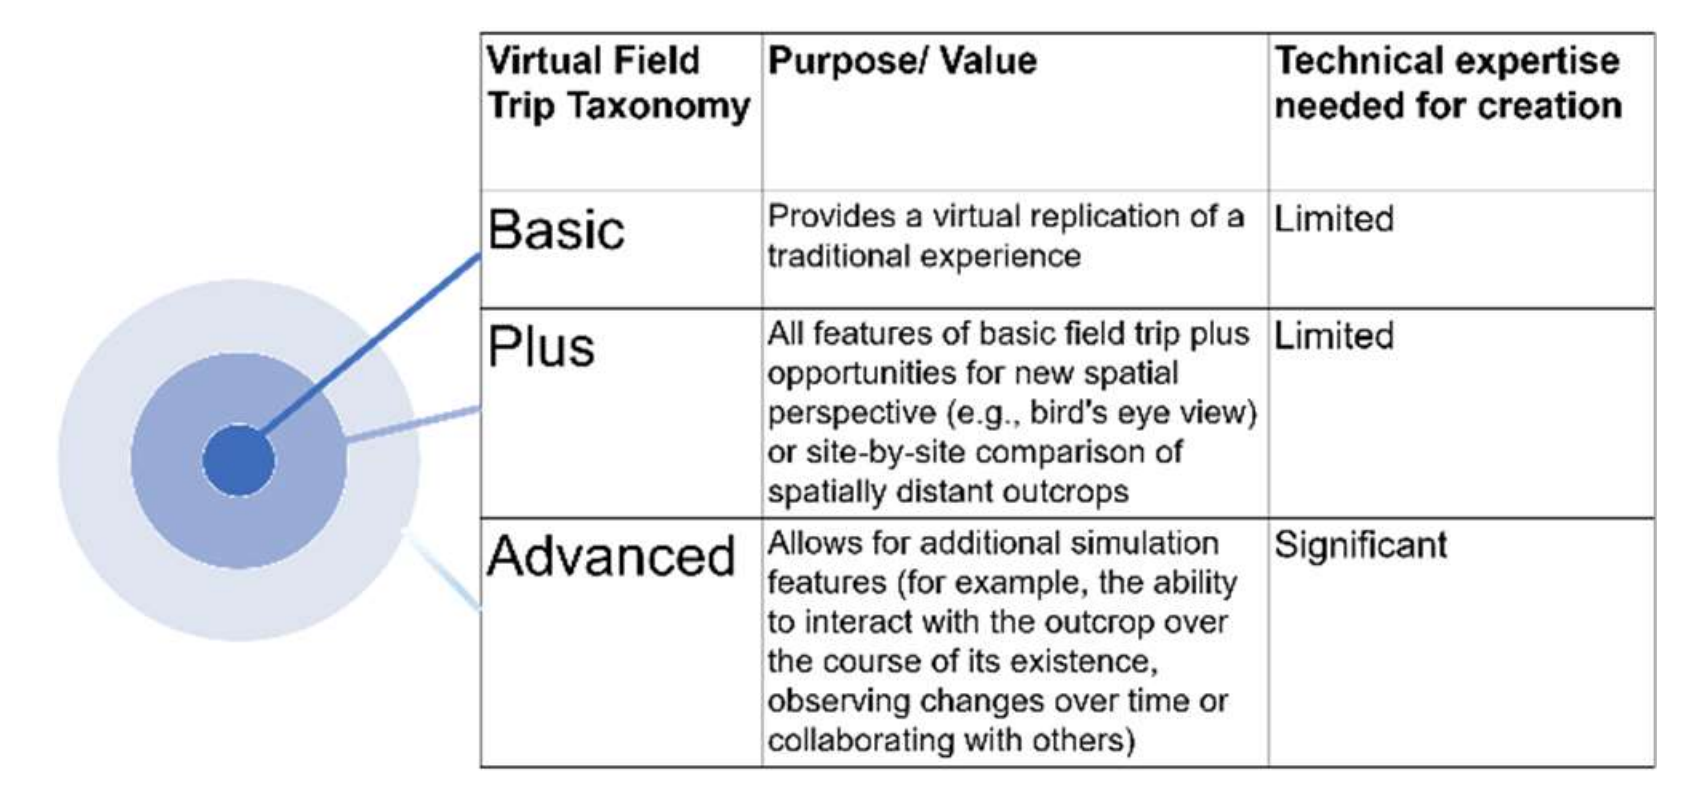
\includegraphics[width=0.7\linewidth]{figures/framework_content_3.PNG}
            \caption{Taxonomy of Immersive Virtual Field Trips}
            \label{fig:taxonomy}
        \end{figure}
        \FloatBarrier
        
        The different levels of Virtual Field Trips are explained in the figure, but can be summed up as Basic being replication of a real field trip, Plus adding new spatial perspective and Advanced adding simulations and / or models, allowing access to realities that does not exist in the real field trip.
        
    \subsection{The LEAGUE Framework for Evaluation}
        \label{sec:league}
        The LEAGUE framework\cite{league} was developed to simplify the evaluation of game-based learning. The framework was created by reading literature on the topic and extracting common features. The features were then placed in a three level hierarchy. The gist of the framework is that game-based learning can be divided into six dimensions (that make up the name LEAGUE): \textbf{L}earning, \textbf{E}nvironment, \textbf{A}ffective Relations, \textbf{G}ame Factors, \textbf{U}sability and Us\textbf{E}r. These dimensions are then further decomposed into factors and sub-factors. Finally, the sub-factors can be evaluated through metrics. The metrics is the lowest level in the model and the parts that can actually be compared. The five metric types are: scores, time, number of occurrences, rating or opinions. The idea of the framework is to use this hierarchical model when planning, designing and evaluating games to ensure a universal language. An overview of the hierarchy is presented in \cref{fig:league}:
        
        \FloatBarrier
        \begin{figure}[htbp]
            \centering
            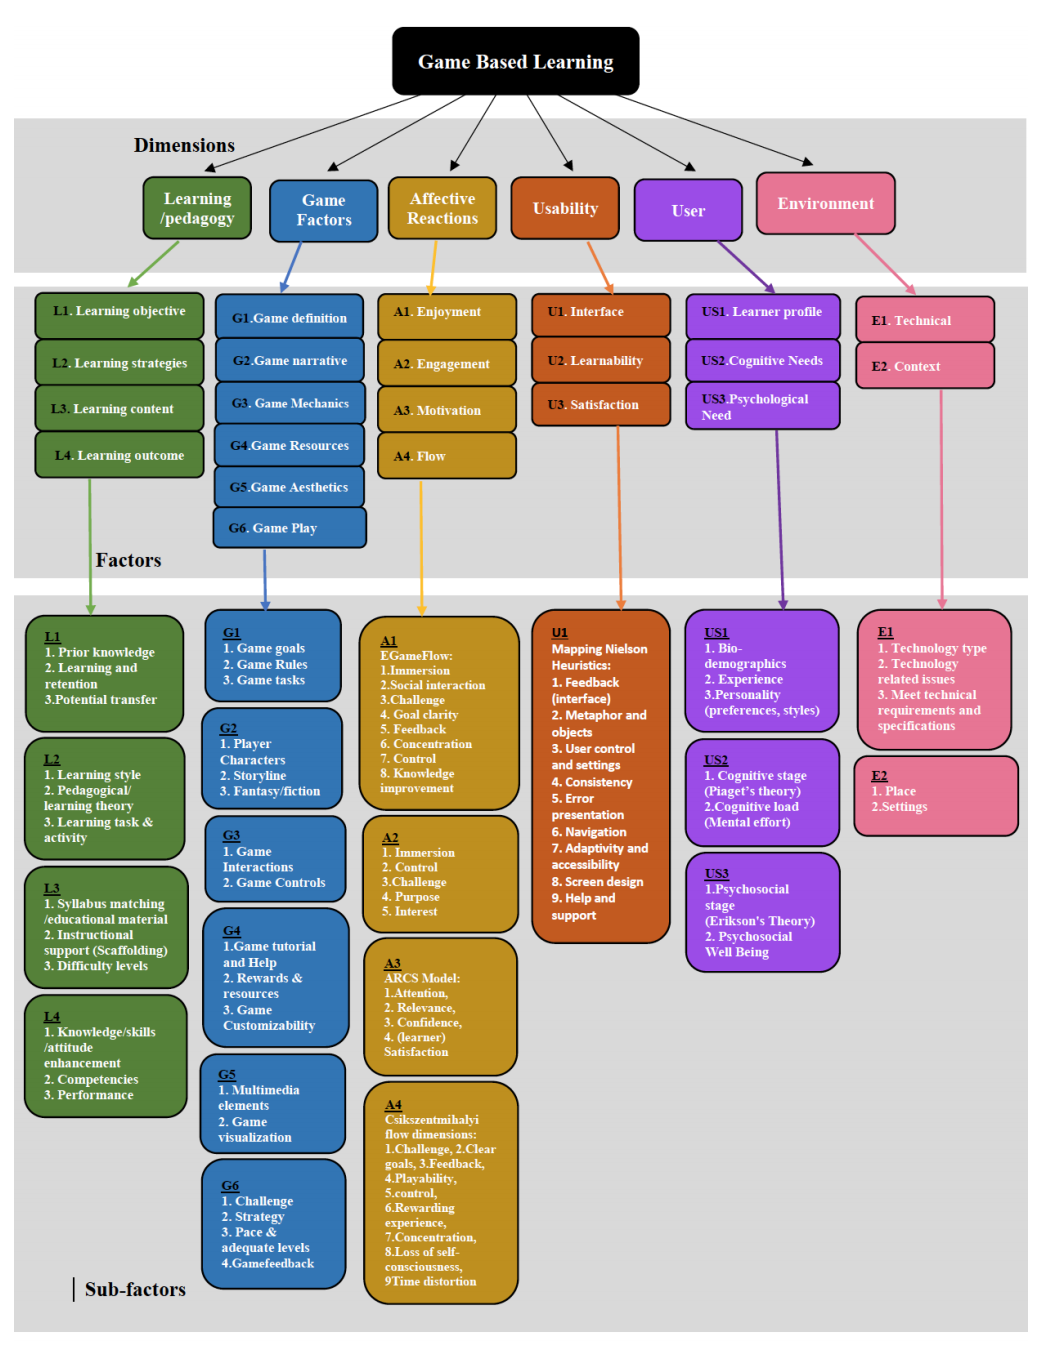
\includegraphics[width=\linewidth]{figures/league.PNG}
            \caption{LEAGUE Hierarchical Structure and Components}
            \label{fig:league}
        \end{figure}
        \FloatBarrier
        
    \subsection{LiDAR}
        A LiDAR scanner is a Light Detection And Ranging equipment that can record the surface area of objects \cite{lidar}. The LiDAR consists of a laser emitter to send laser pulses, a scanner to precisely record the reflected laser pulses, and a GPS receiver to accurately track the position of the LiDAR equipment during scanning. By very precisely recording the time between laser pulses that are sent out and reflected back, the speed of the pulses (light speed) can be used to calculate the distance between the LiDAR and the object reflecting the laser. By repeating this process of sending and detecting laser pulses in different directions, a point cloud will be generated that represent the surface area of the object. Because of the GPS receiver the LiDAR can be moved during scanning, which allows for aerial scanning from helicopters and planes.
        
        LiDAR equipment can be divided into two categories depending on the laser type they use to scan the surfaces. \emph{Topographic} LiDAR systems uses near-infrared lasers. This type of laser will, as explained above, be reflected by surfaces and give a point cloud reminiscent of what one would see from the point of view of the LiDAR. \emph{Bathymetric} LiDAR uses a green light laser. This laser is better at penetrating water, opening the possibilities for mapping sea- and riverbeds where the topographic LiDAR would only return the surface of the water.
        
        As LiDAR equipment bases its sensoring on laser pulses it can also exploit one of the properties of light: not everything is reflected\cite{lidar_canopy}. Illustrated in \cref{fig:transmission} is the effect when some of the light from the LiDAR is reflected back while the rest continues, penetrating through the object or missing it entirely. This is especially common in vegetation, as leaves are thin and do not cover the entire area. This allows one pulse to give multiple readings, which can be used to gather information about the vegetation itself or filter it out to get an isolated view of the ground.
        
        \FloatBarrier
        \begin{figure}[ht]
            \centering
            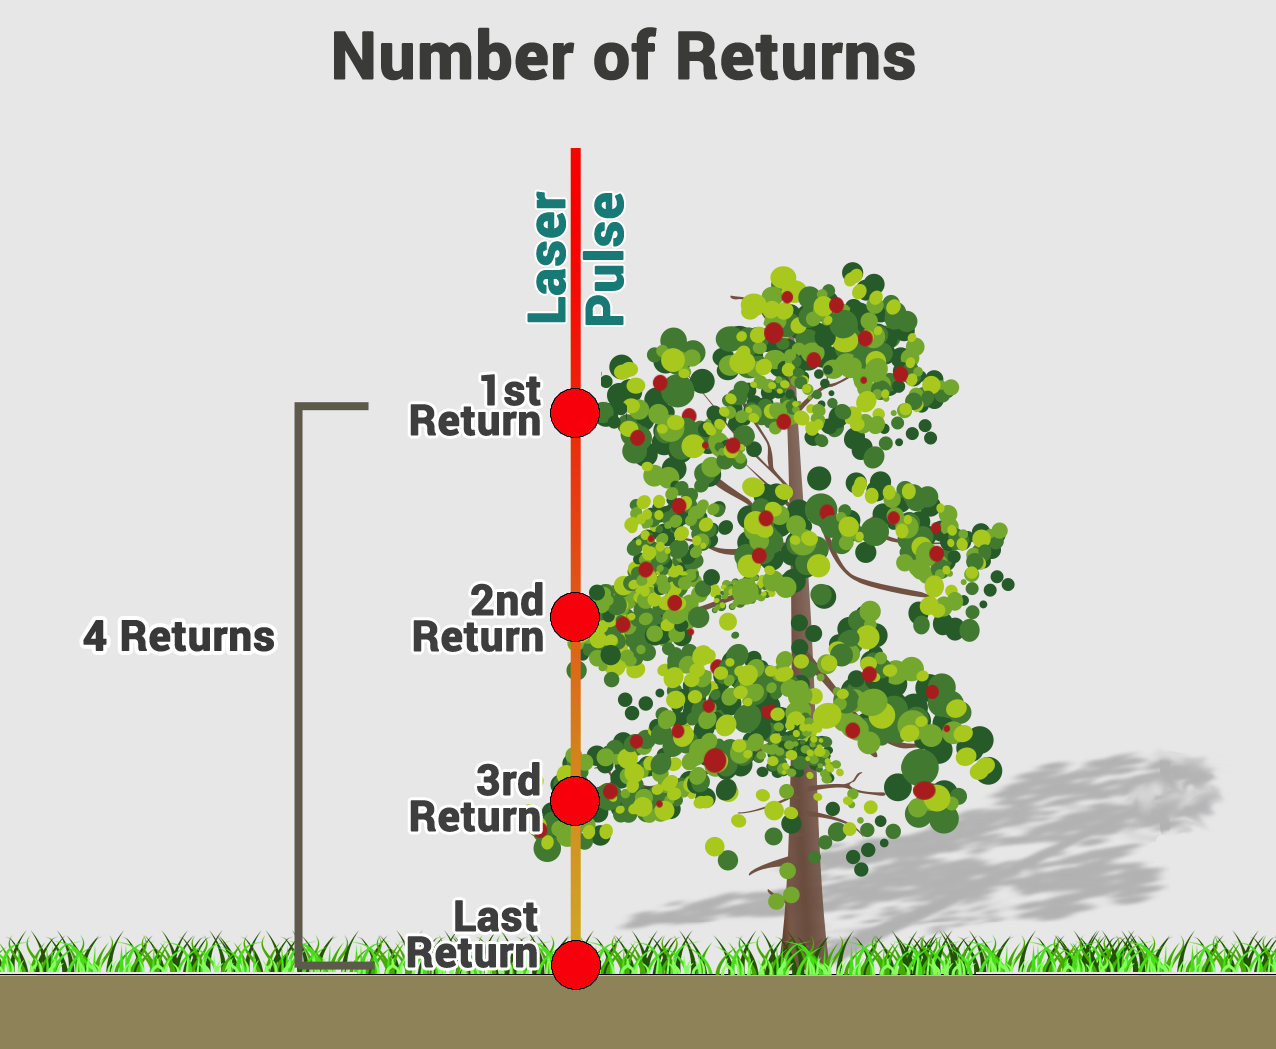
\includegraphics[width=0.5\linewidth]{figures/lidar.png}
            \caption{Laser pulses partially reflecting on- and penetrating canopy}
            \label{fig:transmission}
        \end{figure}
        \FloatBarrier
        %It does this by sending out laser pulses and record the time when they are reflected back in order to determine the distance to a point on a surface. By repeating this process a point cloud can be constructed. LiDAR equipment also record the GPS location for each pulse, which makes it possible to move the scanner during recording and thus open up the possibilities of aerial scans using planes.
        
\section{Game Design}
\label{sec:game_design}
    As the new application is planned to contain interactive elements and meant to be engaging, some theories from Game Design are presented. These are theories and heuristics for creating good games in general, as well as more specific theory related to educational games, which one can argue also adhere to Virtual Field Trips.
        
    \subsection{Lazzaro's Four Fun Keys}
        In chapter 20 of the book \emph{Game Usability: Advice from the Experts for Advancing the Player Experience}\cite{lazzaro}, Lazzaro presents the theory that there are four types of fun to be found in video games. She goes on to describe that players have a tendency to transition between three of these, which implies that successful games have at least three of the four types of fun present to cater to the players desires throughout the gaming sessions. The four types of fun are:
        
        \begin{itemize}
            \item \textbf{Hard Fun}\\
            This is the type of fun most people think of when talking about video games: the fun of the challenge. It is explained that the Hard Fun follows a cycle where the player meets a challenge and builds up frustration, followed by a phase named \emph{Fiero!} when the player overcomes the challenge. Afterwards comes a phase of relaxation where the player can bask in the glory of their achievements before the cycle starts again. It is important that the challenge is correctly balanced to give the player the right amount of frustration before the \emph{Fiero!}. It is also important to allow the player to ''cool down'' before starting to build up more frustration.
            
            \FloatBarrier
            \begin{figure}[ht]
                \centering
                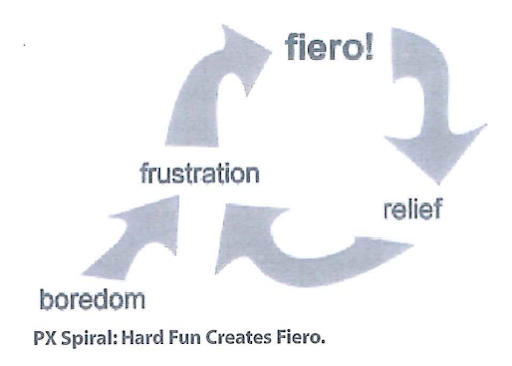
\includegraphics[width=0.5\linewidth]{figures/hard_fun.png}
                \caption{The Hard Fun Cycle}
                \label{fig:hard_fun}
            \end{figure}
            \FloatBarrier
            
            \item \textbf{Easy Fun}\\
            This type of fun is connected to the story and the wonders of the world within the game. It is the type of fun one have when exploring mystic worlds or the curiosity when trying to uncover the hidden story of a forgotten incident. Like the Hard Fun, Easy Fun is also a cyclic behaviour where curiosity leads to a surprise that causes wonder. This is followed by a cool-down phase of relief before the cycle continues. Also similar to Hard Fun, the surprise in Easy Fun must be balanced in order to keep the content familiar enough to be engaging, but also surprising enough.
            
            \FloatBarrier
            \begin{figure}[ht]
                \centering
                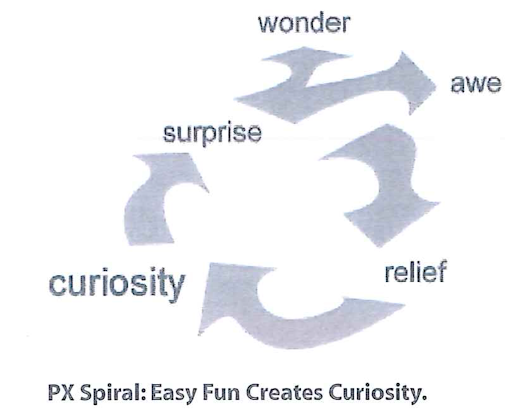
\includegraphics[width=0.5\linewidth]{figures/easy_fun.png}
                \caption{The Easy Fun cycle}
                \label{fig:easy_fun}
            \end{figure}
            \FloatBarrier
            
            \item \textbf{Serious Fun}\\
            This type of fun is defined as when the game ''create something of value outside of the game itself''. Examples of this can be to use games to relax after a hard day at work, to learn rhythms or, in our case, to learn something. Serious Fun can lead to more motivation as the game is not just played for fun, but can improve the player in some way.
            
            \SPACE
            
            \item \textbf{People Fun}\\
            People Fun is the fun related to the social aspects of games. This type of fun is very obvious in multiplayer games with both cooperative and competitive interaction between the players. It does however not explicitly require other players, as it can also be achieved through the use of Non-Player Characters (NPCs).
        \end{itemize}
        
    \subsection{Heuristics For Designing Instructional Computer Games}
        A set of heuristics for designing instructional computer games are given by Malone in his article from 1980\cite{heuristics}. The heuristics describe essential characteristics divided into three categories:
        
        \begin{itemize}
            \item \textbf{Challenge}\\
            Similar to Lazzaro, Malone states that an instructional game must be challenging. He goes forth to describe heuristics for the goal that shall be completed, stating that it should be:
            
            \begin{itemize}
                \item Obvious
                
                \item Compelling
                
                \item Of the appropriate difficulty
                
                \item Offering performance feedback
            \end{itemize}
            
            \SPACE
            
            By following this heuristic the player should end up with knowing what to do, as well as having a motivation for doing it. It should be within the players ability to do it, and they should have a clear indication of how well they perform, both when under- and over performing.
            
            In addition to the goal, the game should have an uncertain outcome. This is to ensure that it becomes exciting, as a game where one always win or always lose can quickly become boring. This uncertain outcome can be achieved by having:
            
            \begin{itemize}
                \item Variable difficulty setting
                
                \item Multiple level goals
                
                \item Hidden information
                
                \item Some randomness
            \end{itemize}
            
            \SPACE
            
            The difficulty can be set manually by the player, or be set automatically by the performance of the player. The difficulty is important as it can greatly affect the self-esteem of the player, which again will influence motivation. Having multiple level goals is another way to balance the difficulty, by making obligatory tasks of the goal easy, but offering challenging optional goals. The hidden information is also a great way to make the outcome of the challenge uncertain by revealing information along the way. Randomness can both aid the hidden information, as well as increasing the difficulty.
            
            \SPACE
            
            \item \textbf{Fantasy}\\
            Fantasy in games can be used to make them more compelling, but can also be used as a means of challenge by having tasks that require players to use their fantasy. An important note is that different fantasies are compelling to different people, and should therefore be chosen based on the target audience.
            
            Malone differs between two different kinds of fantasies: extrinsic and intrinsic. The extrinsic fantasy is dependent on the player skill, where the example in the article is the game Hangman where the visuals depend on the actions of the player. The extrinsic fantasy is also dependant on the skill, but the skill is also dependant on the fantasy. This means that the fantasy is used together with the skill. The example here is a game of darts where the trajectory, angles and force must be fantasised by the player, thus being used in conjunction with the skill.
            
            Emotion is also discussed under the Fantasy category. It is a very powerful element, but it is also very hard to use. By emotionally engaging the player with e.g. NPCs in the game, the goal can be perceived as more compelling, and the feedback will have a stronger impact on the player. Because of the difficulties of using emotion, there are no general way to approach this element.
            
            \SPACE
            
            \item \textbf{Curiosity}\\
            Curiosity mainly stems from having the right amount of \emph{informal complexity}. The goal is to have the player comprehend the situation, but also having some uncertain or hidden information. Curiosity is divided into two categories: sensory and cognitive. The sensory curiosity instinctively captures the players attention, usually by playing visual or audible ques. This plays on the ''lizard brain'' of humans that automatically seeks out movement and flashing lights. The cognitive curiosity however relies on missing information. This has some similarities with Lazzaro's Easy Fun in that the missing information should be surprising to engage the player and motivate further progress.
        \end{itemize}

\section{Existing Solutions}
    % Products of Virtual Field Trips that are available to be used atm
    
    \todo{Include images of applications?}
    
    As discussed in \cref{sec:motivation}, virtual field trips using VR is already present and available as commercial products. A quick introduction to some of the most similar or relevant solutions are presented, as well as summary comparing the different applications on key factors. The solutions were identified and described in the Specialisation Project\cite{specialisation}. Applications are chosen based on the criteria below, where the first is mandatory and at least one of the other two must be present.
    
    \begin{itemize}
        \item \textbf{Application have to be in VR}
        
        \item Application is a Virtual Field Trip
        
        \item Applications uses an omnidirectional treadmill
    \end{itemize}
    
    \subsection{Penn State University Application}
        Penn State University has created an application for showing images taken from a field course. The application provides the player with an aerial map of the area where image locations are highlighted. Players can then select images from the map, from a menu available when in image mode and by using arrows within the image to move to adjacent images. The application only support monoscopic 360 images, limited by the intended hardware: Oculus Go and Oculus Quest. The application does allow for multiple users at the same time, where one of the users can guide the other users through the images while explaining the content.
        
        This is the Virtual Field Trip that will be used to compare and evaluate the new application. It has been made in collaboration with Penn State. Specifications for how to capture and mark the footage was supplied from Penn State and the images were sent back in monoscopic format, geotagged and with indications of which images transition to which. The development was incremental with a prototype being tested on domain experts and reworked based on their feedback.
    
    \subsection{Google Expedition}
        % Phone app
        % VR and AR
        % One leader can see where other participants are seeing
        % "Go anywhere with VR, see anything with AR"
        % Create own virtual tours with Tour Creator
        Google Expedition is a smart phone application available on both Google Play and the App Store. As can be read on Google's own pages about the product \cite{google_expeditions}, the application offers both VR and AR functions. When used as VR, one leader can guide others through 360 images and see where the participants are looking. When using the AR functionalities, objects can be displayed and viewed from all angles making the participants walk around a fixed physical location in the classroom.
        
        Google Expedition also has the ability for domain experts to create their own Virtual Field Trips with the Tour Creator. It can create tours from 360 images, 180 images or images from Google Street View.
    
    \subsection{Google Earth VR}
        Google Earth VR is another VR application by Google and is described on their website\cite{google_earth_vr}. It creates a 3D model from satellite imagery that the user can traverse. It is however, in line with their 2D application Google Earth, a service that does not allow the user to scale up or zoom in to a human sized perception. Because of this its model recreation is also somewhat coarse, working best when reproducing larger objects like mountains and valleys.
    
    \subsection{Climate Quest and Player Program}
        One of the most recent papers produced about the Virtuix Omni is a bachelor project from NTNU \cite{bachelor}. The team of students created three applications. In \emph{Climate Quest} the player can run around in the Trondheim city centre while the ocean level is rising. The player is tasked with shooting objects with negative impact on the climate, converting them to greener solutions. Shooting the objects also decrease the water level making it safe to navigate the lowest point in the level/area. In addition to the water level rising, points were given for shooting the targets. Points were also based on the time the player used. The team also performed user tests, which gave very positive feedback. The tests were primarily centred around testing the application, not if the user changed their feelings towards climate change.
        
        The Bachelor project also included an application for shooting generic targets, called Player Program. The targets can either only give points, or display text as well. The application is meant as an educational tool where the text can display knowledge to help students learn. Like the Climate Quest, this application also takes time into consideration when calculating points to create a more engaging experience.
        
        The third application is a desktop application for placing the targets for the learning tool mentioned above. This allows e.g. a professor to place the targets and assign custom text to some of them. This will then be exported as a \texttt{.json} file that can be imported by the learning tool application. This is an important tool as it bridges the gap between domain experts and software development, although it is currently only available for the Trondheim city centre.
        
    \subsection{Stanford Ocean Acidification}
        Another application that explores climate change comes from Stanford University\cite{virtual_field_trips_learning}. In the experiment the effect of the Virtual Field Trip as a medium for learning about ocean acidification is explored. This is one of the more interactive applications that were found, consisting of four studies with four different applications or versions of applications. The user is placed underwater and can interact with the environment like fishes and corals. Depending on the application the user also have one of several avatars to represent their body in the application. The interactions are related to the nature of the Virtual Field Trip, with some of them being counting species with a time limit in different environments. Another of the applications have the user embody a coral and have to collect calcium bicarbonate ions from the water in order to grow. Another test that was conducted was to have a fish bump into the player while a person taps the player gently in real life with an object to simulate the feel of the fish. A common denominator between the applications used is that the user is stationary in the in-game world.
        
    \subsection{Inland Simulated Nature Walk}
        The research at the Inland University, discussed in \cref{sec:vft} - Virtual Field Trips, produced an application based on 360$^{\circ}$ video. Although it might not be considered a virtual field trip, it was included because of its work on reconstructing a real area. The simulated nature walk\cite{ive} could either be experienced while sitting down, or while walking on a one-directional, mechanical treadmill. A 360$^{\circ}$ video of walking along a trail plays in its entirety and, in the case of the treadmill, the walking speed is determined by the user. The application did not have any controller input.
        
    \subsection{The Virtual UCF Arboretum}
        Created by the University of Central Florida (\todo{cite?}), the Virtual UCF Arboretum\cite{florida_vft} is a highly detailed virtual recreation of wild nature. The different botanical models in the application are of high precision and created to be as realistic and correct as possible. Different tools were used to achieve the high details, like historic geographic information system (GIS) data, field observations, images, measurements and drone footage. The application is also integrated with a website, offering more information on e.g. different tree species. It also offers different modes of transportation, like walking, teleporting and flying. The flying allows the player get different point of view of the area.
        
    \subsection{Summary}
        \label{sec:summary}
        In order to compare the different solutions, they are placed on the two dimensional axis of the research framework presented in \cref{sec:framework}. The sensing part of this framework is interpreted as low having only head tracking, medium having head- and hand tracking, and advanced tracking more than medium. They are also compared on whether or not they use real images, and if they have replicated a real area in the form of a model. The solutions are also marked depending on if they are a Virtual Field Trip(VFT) or not.
    
        \FloatBarrier
        \begin{table}[htbp]
            \centering
            \caption{Comparison of Existing Solutions}
            \label{tab:comparison}
            \begin{tabularx}{\linewidth}{| >{\raggedright\arraybackslash}X | >{\centering\arraybackslash}X | >{\centering\arraybackslash}X | >{\centering\arraybackslash}X | >{\centering\arraybackslash}X | >{\centering\arraybackslash}X |}
                \hline
                \textbf{Solution} & \textbf{Sensing} & \textbf{Taxonomy} & \textbf{Replication} & \textbf{Images} & \textbf{VFT} \\
                \hline
                Penn State University Application & Low & Basic & No & Yes & Yes \\
                Google Expedition & Low & Basic & No & Yes & Yes \\
                Google Earth VR & Low & Plus & Yes & Yes & No \\
                Climate Quest & High & Advanced & Yes & No & No \\
                Player Program & High & Advanced & Yes & No & Yes? \\
                Stanford Ocean Acidification & Medium & Advanced & No & No & Yes \\
                Simulated Nature Walk & Low & Basic & No & Yes (video) & No \\
                Virtual UCF Arboretum & Medium & Plus & Yes & No & Yes \\
                \ApplicationName & High & Advanced & Yes & Yes & Yes \\
                \hline
            \end{tabularx}
        \end{table}
        \FloatBarrier
        
        \todo{Colour the comparison table?}
